\documentclass[border=8pt]{standalone}
\usepackage{pgfplots}
\usepgfplotslibrary{groupplots,fillbetween}
\pgfplotsset{compat=1.18}
\renewcommand{\familydefault}{\sfdefault}
\definecolor{oursline}{HTML}{00747C}
\definecolor{omleline}{HTML}{773588}
\definecolor{ink}{HTML}{17242D}
\definecolor{muted}{HTML}{4A5C67}
\definecolor{gridline}{HTML}{E3EAED}
\begin{document}
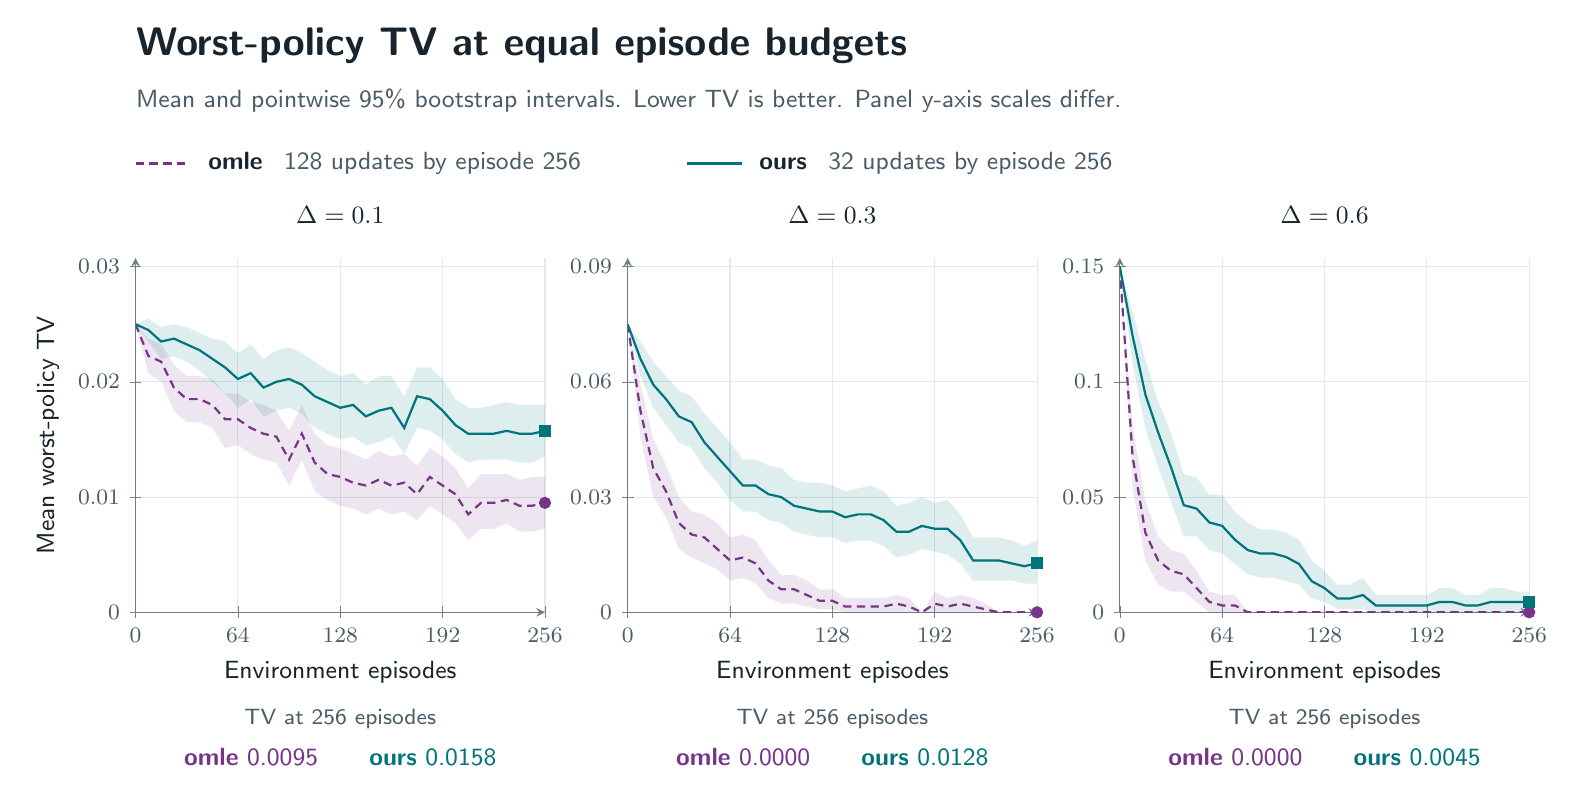
\begin{tikzpicture}[text=ink]
\begin{groupplot}[
  group style={group size=3 by 1,horizontal sep=1.05cm},
  width=5.2cm,height=4.5cm,scale only axis,
  xmin=0,ymin=0,
  xtick={0,64,128,192,256},
  tick align=outside,tick style={muted!75},
  tick label style={font=\footnotesize,text=muted},
  label style={font=\small,text=ink},
  scaled y ticks=false,
  yticklabel style={/pgf/number format/fixed,/pgf/number format/precision=3},
  title style={font=\small\bfseries,text=ink,yshift=1mm},
  grid=major,grid style={gridline},
  axis lines=left,axis line style={muted!80},
  xlabel={Environment episodes},
]
\nextgroupplot[title={$\Delta=0.1$},xmax=256,ymax=0.030749999999999996,ytick={0,0.01,0.02,0.03},ylabel={Mean worst-policy TV}]
\addplot[draw=none,name path=omle1low] coordinates {(0,0.025) (8,0.02075) (16,0.02) (24,0.0175) (32,0.0165) (40,0.0165) (48,0.016) (56,0.01425) (64,0.0145) (72,0.01375) (80,0.01325) (88,0.013) (96,0.011) (104,0.01325) (112,0.0105) (120,0.00974375) (128,0.00925) (136,0.009) (144,0.0085) (152,0.009) (160,0.0085) (168,0.00875) (176,0.00799375) (184,0.00925) (192,0.0085) (200,0.00775) (208,0.00625) (216,0.00725) (224,0.00725) (232,0.00774375) (240,0.007) (248,0.007) (256,0.00725)};
\addplot[draw=none,name path=omle1high] coordinates {(0,0.025) (8,0.02375) (16,0.02325) (24,0.0215) (32,0.0205) (40,0.0205) (48,0.02025) (56,0.019) (64,0.019) (72,0.01825) (80,0.018) (88,0.01750625) (96,0.01575) (104,0.018) (112,0.0155) (120,0.0145) (128,0.01425) (136,0.01375) (144,0.01325) (152,0.014) (160,0.0135) (168,0.01375) (176,0.01275) (184,0.01425) (192,0.0135) (200,0.0125) (208,0.01075) (216,0.012) (224,0.012) (232,0.012) (240,0.0115) (248,0.01175) (256,0.01175625)};
\addplot[omleline,fill opacity=0.13,draw=none] fill between[of=omle1low and omle1high];
\addplot[draw=none,name path=ours1low] coordinates {(0,0.025) (8,0.0235) (16,0.022) (24,0.02225) (32,0.02174375) (40,0.021) (48,0.02) (56,0.019) (64,0.01775) (72,0.0185) (80,0.017) (88,0.0175) (96,0.01775) (104,0.01725) (112,0.016) (120,0.0155) (128,0.015) (136,0.01525) (144,0.0145) (152,0.01475) (160,0.01525) (168,0.01375) (176,0.016) (184,0.01575) (192,0.01499375) (200,0.01375) (208,0.013) (216,0.01325) (224,0.01324375) (232,0.01325) (240,0.013) (248,0.013) (256,0.0135)};
\addplot[draw=none,name path=ours1high] coordinates {(0,0.025) (8,0.0255) (16,0.02475) (24,0.025) (32,0.02475) (40,0.02425) (48,0.02375) (56,0.0235) (64,0.0225) (72,0.02325) (80,0.022) (88,0.02275) (96,0.023) (104,0.0225) (112,0.02175) (120,0.021) (128,0.0205) (136,0.02075) (144,0.01975) (152,0.0205) (160,0.0205) (168,0.01875) (176,0.02125) (184,0.02125) (192,0.02025) (200,0.01850625) (208,0.01775) (216,0.01775) (224,0.018) (232,0.01825) (240,0.018) (248,0.018) (256,0.018)};
\addplot[oursline,fill opacity=0.13,draw=none] fill between[of=ours1low and ours1high];
\addplot[omleline,thick,densely dashed,mark=none] coordinates {(0,0.025) (8,0.02225) (16,0.02175) (24,0.0195) (32,0.0185) (40,0.0185) (48,0.018) (56,0.01675) (64,0.01675) (72,0.016) (80,0.0155) (88,0.01525) (96,0.01325) (104,0.0155) (112,0.013) (120,0.012) (128,0.01175) (136,0.01125) (144,0.011) (152,0.0115) (160,0.011) (168,0.01125) (176,0.01025) (184,0.01175) (192,0.011) (200,0.01025) (208,0.0085) (216,0.0095) (224,0.0095) (232,0.00975) (240,0.00925) (248,0.00925) (256,0.0095)};
\addplot[only marks,mark=*,mark size=2pt,omleline,clip marker paths=false] coordinates {(256,0.0095)};
\addplot[oursline,thick,solid,mark=none] coordinates {(0,0.025) (8,0.0245) (16,0.0235) (24,0.02375) (32,0.02325) (40,0.02275) (48,0.022) (56,0.02125) (64,0.02025) (72,0.02075) (80,0.0195) (88,0.02) (96,0.02025) (104,0.01975) (112,0.01875) (120,0.01825) (128,0.01775) (136,0.018) (144,0.017) (152,0.0175) (160,0.01775) (168,0.016) (176,0.01875) (184,0.0185) (192,0.0175) (200,0.01625) (208,0.0155) (216,0.0155) (224,0.0155) (232,0.01575) (240,0.0155) (248,0.0155) (256,0.01575)};
\addplot[only marks,mark=square*,mark size=2pt,oursline,clip marker paths=false] coordinates {(256,0.01575)};
\nextgroupplot[title={$\Delta=0.3$},xmax=256,ymax=0.09224999999999998,ytick={0,0.03,0.06,0.09}]
\addplot[draw=none,name path=omle2low] coordinates {(0,0.075) (8,0.04575) (16,0.03) (24,0.02475) (32,0.0165) (40,0.01425) (48,0.01275) (56,0.01123125) (64,0.00825) (72,0.00898125) (80,0.0075) (88,0.00375) (96,0.00225) (104,0.00225) (112,0.0015) (120,0.00075) (128,0.00075) (136,0) (144,0) (152,0) (160,0) (168,0) (176,0) (184,0) (192,0) (200,0) (208,0) (216,0) (224,0) (232,0) (240,0) (248,0) (256,0)};
\addplot[draw=none,name path=omle2high] coordinates {(0,0.075) (8,0.05925) (16,0.045) (24,0.03825) (32,0.03) (40,0.02626875) (48,0.0255) (56,0.02325) (64,0.0195) (72,0.02025) (80,0.01875) (88,0.0135) (96,0.00975) (104,0.00975) (112,0.00825) (120,0.006) (128,0.006) (136,0.00375) (144,0.00375) (152,0.00375) (160,0.00375) (168,0.00451875) (176,0.00375) (184,0) (192,0.00525) (200,0.00375) (208,0.00451875) (216,0.00375) (224,0.00225) (232,0) (240,0) (248,0) (256,0)};
\addplot[omleline,fill opacity=0.13,draw=none] fill between[of=omle2low and omle2high];
\addplot[draw=none,name path=ours2low] coordinates {(0,0.075) (8,0.06148125) (16,0.05325) (24,0.04875) (32,0.04425) (40,0.04275) (48,0.0375) (56,0.03373125) (64,0.02925) (72,0.02625) (80,0.02623125) (88,0.024) (96,0.02325) (104,0.021) (112,0.02023125) (120,0.0195) (128,0.0195) (136,0.018) (144,0.01875) (152,0.01875) (160,0.01725) (168,0.01425) (176,0.015) (184,0.0165) (192,0.01575) (200,0.015) (208,0.01275) (216,0.00825) (224,0.00825) (232,0.00825) (240,0.00825) (248,0.0075) (256,0.0075)};
\addplot[draw=none,name path=ours2high] coordinates {(0,0.075) (8,0.0705) (16,0.06525) (24,0.0615) (32,0.05775) (40,0.05625) (48,0.05175) (56,0.048) (64,0.04425) (72,0.03976875) (80,0.03975) (88,0.03825) (96,0.0375) (104,0.0345) (112,0.03375) (120,0.03375) (128,0.033) (136,0.03151875) (144,0.03225) (152,0.033) (160,0.0315) (168,0.02775) (176,0.0285) (184,0.03) (192,0.02851875) (200,0.02925) (208,0.0255) (216,0.0195) (224,0.0195) (232,0.0195) (240,0.01875) (248,0.01725) (256,0.01875)};
\addplot[oursline,fill opacity=0.13,draw=none] fill between[of=ours2low and ours2high];
\addplot[omleline,thick,densely dashed,mark=none] coordinates {(0,0.075) (8,0.0525) (16,0.0375) (24,0.0315) (32,0.02325) (40,0.02025) (48,0.0195) (56,0.0165) (64,0.0135) (72,0.01425) (80,0.01275) (88,0.00825) (96,0.006) (104,0.006) (112,0.0045) (120,0.003) (128,0.003) (136,0.0015) (144,0.0015) (152,0.0015) (160,0.0015) (168,0.00225) (176,0.0015) (184,0) (192,0.00225) (200,0.0015) (208,0.00225) (216,0.0015) (224,0.00075) (232,0) (240,0) (248,0) (256,0)};
\addplot[only marks,mark=*,mark size=2pt,omleline,clip marker paths=false] coordinates {(256,0)};
\addplot[oursline,thick,solid,mark=none] coordinates {(0,0.075) (8,0.066) (16,0.05925) (24,0.0555) (32,0.051) (40,0.0495) (48,0.04425) (56,0.0405) (64,0.03675) (72,0.033) (80,0.033) (88,0.03075) (96,0.03) (104,0.02775) (112,0.027) (120,0.02625) (128,0.02625) (136,0.02475) (144,0.0255) (152,0.0255) (160,0.024) (168,0.021) (176,0.021) (184,0.0225) (192,0.02175) (200,0.02175) (208,0.01875) (216,0.0135) (224,0.0135) (232,0.0135) (240,0.01275) (248,0.012) (256,0.01275)};
\addplot[only marks,mark=square*,mark size=2pt,oursline,clip marker paths=false] coordinates {(256,0.01275)};
\nextgroupplot[title={$\Delta=0.6$},xmax=256,ymax=0.15374999999999997,ytick={0,0.05,0.10,0.15}]
\addplot[draw=none,name path=omle3low] coordinates {(0,0.15) (8,0.054) (16,0.0225) (24,0.012) (32,0.009) (40,0.009) (48,0.0045) (56,0) (64,0) (72,0) (80,0) (88,0) (96,0) (104,0) (112,0) (120,0) (128,0) (136,0) (144,0) (152,0) (160,0) (168,0) (176,0) (184,0) (192,0) (200,0) (208,0) (216,0) (224,0) (232,0) (240,0) (248,0) (256,0)};
\addplot[draw=none,name path=omle3high] coordinates {(0,0.15) (8,0.081) (16,0.048) (24,0.033) (32,0.027) (40,0.0255) (48,0.018) (56,0.009) (64,0.0075) (72,0.0075) (80,0) (88,0) (96,0) (104,0) (112,0) (120,0) (128,0) (136,0) (144,0) (152,0) (160,0) (168,0) (176,0) (184,0) (192,0) (200,0) (208,0) (216,0) (224,0) (232,0) (240,0) (248,0) (256,0)};
\addplot[omleline,fill opacity=0.13,draw=none] fill between[of=omle3low and omle3high];
\addplot[draw=none,name path=ours3low] coordinates {(0,0.15) (8,0.108) (16,0.0795) (24,0.063) (32,0.048) (40,0.033) (48,0.033) (56,0.027) (64,0.0255) (72,0.0209625) (80,0.0165) (88,0.015) (96,0.015) (104,0.0135) (112,0.012) (120,0.006) (128,0.0045) (136,0.0015) (144,0.0015) (152,0.0015) (160,0) (168,0) (176,0) (184,0) (192,0) (200,0) (208,0) (216,0) (224,0) (232,0) (240,0) (248,0) (256,0)};
\addplot[draw=none,name path=ours3high] coordinates {(0,0.15) (8,0.1305) (16,0.1095) (24,0.0915) (32,0.078) (40,0.06) (48,0.0585) (56,0.0510375) (64,0.051) (72,0.0435) (80,0.039) (88,0.036) (96,0.036) (104,0.0345) (112,0.0315) (120,0.0225) (128,0.018) (136,0.012) (144,0.012) (152,0.015) (160,0.0075) (168,0.0075) (176,0.0075) (184,0.0075) (192,0.0075) (200,0.0105) (208,0.0105) (216,0.0075) (224,0.0075) (232,0.0105) (240,0.0105) (248,0.009) (256,0.009)};
\addplot[oursline,fill opacity=0.13,draw=none] fill between[of=ours3low and ours3high];
\addplot[omleline,thick,densely dashed,mark=none] coordinates {(0,0.15) (8,0.0675) (16,0.0345) (24,0.0225) (32,0.018) (40,0.0165) (48,0.0105) (56,0.0045) (64,0.003) (72,0.003) (80,0) (88,0) (96,0) (104,0) (112,0) (120,0) (128,0) (136,0) (144,0) (152,0) (160,0) (168,0) (176,0) (184,0) (192,0) (200,0) (208,0) (216,0) (224,0) (232,0) (240,0) (248,0) (256,0)};
\addplot[only marks,mark=*,mark size=2pt,omleline,clip marker paths=false] coordinates {(256,0)};
\addplot[oursline,thick,solid,mark=none] coordinates {(0,0.15) (8,0.12) (16,0.0945) (24,0.078) (32,0.063) (40,0.0465) (48,0.045) (56,0.039) (64,0.0375) (72,0.0315) (80,0.027) (88,0.0255) (96,0.0255) (104,0.024) (112,0.021) (120,0.0135) (128,0.0105) (136,0.006) (144,0.006) (152,0.0075) (160,0.003) (168,0.003) (176,0.003) (184,0.003) (192,0.003) (200,0.0045) (208,0.0045) (216,0.003) (224,0.003) (232,0.0045) (240,0.0045) (248,0.0045) (256,0.0045)};
\addplot[only marks,mark=square*,mark size=2pt,oursline,clip marker paths=false] coordinates {(256,0.0045)};
\end{groupplot}
\node[anchor=west,inner sep=0pt,font=\bfseries\Large] at ([yshift=27mm]group c1r1.north west) {Worst-policy TV at equal episode budgets};
\node[anchor=west,inner sep=0pt,text=muted,font=\small] at ([yshift=20mm]group c1r1.north west) {Mean and pointwise 95\% bootstrap intervals. Lower TV is better. Panel y-axis scales differ.};
\draw[omleline,very thick,densely dashed] ([xshift=0mm,yshift=12mm]group c1r1.north west) -- ++(7mm,0);
\node[anchor=west,font=\small] at ([xshift=8mm,yshift=12mm]group c1r1.north west) {\textbf{omle} \enspace \textcolor{muted}{128 updates by episode 256}};
\draw[oursline,very thick,solid] ([xshift=70mm,yshift=12mm]group c1r1.north west) -- ++(7mm,0);
\node[anchor=west,font=\small] at ([xshift=78mm,yshift=12mm]group c1r1.north west) {\textbf{ours} \enspace \textcolor{muted}{32 updates by episode 256}};
\node[anchor=north,font=\footnotesize,text=muted] at ([yshift=-11mm]group c1r1.south) {TV at 256 episodes};
\node[anchor=north,font=\small] at ([yshift=-16mm]group c1r1.south) {\textcolor{omleline}{\textbf{omle} 0.0095}\qquad \textcolor{oursline}{\textbf{ours} 0.0158}};
\node[anchor=north,font=\footnotesize,text=muted] at ([yshift=-11mm]group c2r1.south) {TV at 256 episodes};
\node[anchor=north,font=\small] at ([yshift=-16mm]group c2r1.south) {\textcolor{omleline}{\textbf{omle} 0.0000}\qquad \textcolor{oursline}{\textbf{ours} 0.0128}};
\node[anchor=north,font=\footnotesize,text=muted] at ([yshift=-11mm]group c3r1.south) {TV at 256 episodes};
\node[anchor=north,font=\small] at ([yshift=-16mm]group c3r1.south) {\textcolor{omleline}{\textbf{omle} 0.0000}\qquad \textcolor{oursline}{\textbf{ours} 0.0045}};
\end{tikzpicture}
\end{document}
